% Options for packages loaded elsewhere
\PassOptionsToPackage{unicode}{hyperref}
\PassOptionsToPackage{hyphens}{url}
%
\documentclass[
]{article}
\usepackage{lmodern}
\usepackage{amssymb,amsmath}
\usepackage{ifxetex,ifluatex}
\ifnum 0\ifxetex 1\fi\ifluatex 1\fi=0 % if pdftex
  \usepackage[T1]{fontenc}
  \usepackage[utf8]{inputenc}
  \usepackage{textcomp} % provide euro and other symbols
\else % if luatex or xetex
  \usepackage{unicode-math}
  \defaultfontfeatures{Scale=MatchLowercase}
  \defaultfontfeatures[\rmfamily]{Ligatures=TeX,Scale=1}
\fi
% Use upquote if available, for straight quotes in verbatim environments
\IfFileExists{upquote.sty}{\usepackage{upquote}}{}
\IfFileExists{microtype.sty}{% use microtype if available
  \usepackage[]{microtype}
  \UseMicrotypeSet[protrusion]{basicmath} % disable protrusion for tt fonts
}{}
\makeatletter
\@ifundefined{KOMAClassName}{% if non-KOMA class
  \IfFileExists{parskip.sty}{%
    \usepackage{parskip}
  }{% else
    \setlength{\parindent}{0pt}
    \setlength{\parskip}{6pt plus 2pt minus 1pt}}
}{% if KOMA class
  \KOMAoptions{parskip=half}}
\makeatother
\usepackage{xcolor}
\IfFileExists{xurl.sty}{\usepackage{xurl}}{} % add URL line breaks if available
\IfFileExists{bookmark.sty}{\usepackage{bookmark}}{\usepackage{hyperref}}
\hypersetup{
  pdftitle={Just say hello!},
  pdfauthor={My Friend},
  hidelinks,
  pdfcreator={LaTeX via pandoc}}
\urlstyle{same} % disable monospaced font for URLs
\usepackage{color}
\usepackage{fancyvrb}
\newcommand{\VerbBar}{|}
\newcommand{\VERB}{\Verb[commandchars=\\\{\}]}
\DefineVerbatimEnvironment{Highlighting}{Verbatim}{commandchars=\\\{\}}
% Add ',fontsize=\small' for more characters per line
\newenvironment{Shaded}{}{}
\newcommand{\AlertTok}[1]{\textcolor[rgb]{1.00,0.00,0.00}{\textbf{#1}}}
\newcommand{\AnnotationTok}[1]{\textcolor[rgb]{0.38,0.63,0.69}{\textbf{\textit{#1}}}}
\newcommand{\AttributeTok}[1]{\textcolor[rgb]{0.49,0.56,0.16}{#1}}
\newcommand{\BaseNTok}[1]{\textcolor[rgb]{0.25,0.63,0.44}{#1}}
\newcommand{\BuiltInTok}[1]{#1}
\newcommand{\CharTok}[1]{\textcolor[rgb]{0.25,0.44,0.63}{#1}}
\newcommand{\CommentTok}[1]{\textcolor[rgb]{0.38,0.63,0.69}{\textit{#1}}}
\newcommand{\CommentVarTok}[1]{\textcolor[rgb]{0.38,0.63,0.69}{\textbf{\textit{#1}}}}
\newcommand{\ConstantTok}[1]{\textcolor[rgb]{0.53,0.00,0.00}{#1}}
\newcommand{\ControlFlowTok}[1]{\textcolor[rgb]{0.00,0.44,0.13}{\textbf{#1}}}
\newcommand{\DataTypeTok}[1]{\textcolor[rgb]{0.56,0.13,0.00}{#1}}
\newcommand{\DecValTok}[1]{\textcolor[rgb]{0.25,0.63,0.44}{#1}}
\newcommand{\DocumentationTok}[1]{\textcolor[rgb]{0.73,0.13,0.13}{\textit{#1}}}
\newcommand{\ErrorTok}[1]{\textcolor[rgb]{1.00,0.00,0.00}{\textbf{#1}}}
\newcommand{\ExtensionTok}[1]{#1}
\newcommand{\FloatTok}[1]{\textcolor[rgb]{0.25,0.63,0.44}{#1}}
\newcommand{\FunctionTok}[1]{\textcolor[rgb]{0.02,0.16,0.49}{#1}}
\newcommand{\ImportTok}[1]{#1}
\newcommand{\InformationTok}[1]{\textcolor[rgb]{0.38,0.63,0.69}{\textbf{\textit{#1}}}}
\newcommand{\KeywordTok}[1]{\textcolor[rgb]{0.00,0.44,0.13}{\textbf{#1}}}
\newcommand{\NormalTok}[1]{#1}
\newcommand{\OperatorTok}[1]{\textcolor[rgb]{0.40,0.40,0.40}{#1}}
\newcommand{\OtherTok}[1]{\textcolor[rgb]{0.00,0.44,0.13}{#1}}
\newcommand{\PreprocessorTok}[1]{\textcolor[rgb]{0.74,0.48,0.00}{#1}}
\newcommand{\RegionMarkerTok}[1]{#1}
\newcommand{\SpecialCharTok}[1]{\textcolor[rgb]{0.25,0.44,0.63}{#1}}
\newcommand{\SpecialStringTok}[1]{\textcolor[rgb]{0.73,0.40,0.53}{#1}}
\newcommand{\StringTok}[1]{\textcolor[rgb]{0.25,0.44,0.63}{#1}}
\newcommand{\VariableTok}[1]{\textcolor[rgb]{0.10,0.09,0.49}{#1}}
\newcommand{\VerbatimStringTok}[1]{\textcolor[rgb]{0.25,0.44,0.63}{#1}}
\newcommand{\WarningTok}[1]{\textcolor[rgb]{0.38,0.63,0.69}{\textbf{\textit{#1}}}}
\setlength{\emergencystretch}{3em} % prevent overfull lines
\providecommand{\tightlist}{%
  \setlength{\itemsep}{0pt}\setlength{\parskip}{0pt}}
\setcounter{secnumdepth}{-\maxdimen} % remove section numbering
\usepackage{tikz,pgfplots}
\usepackage{fancyhdr}
\pagestyle{fancy}
\fancyhead[CO,CE]{This is fancy}
\fancyfoot[CO,CE]{So is this}
\fancyfoot[LE,RO]{\thepage}

\title{Just say hello!}
\author{My Friend}
\date{}

\begin{document}
\maketitle
\begin{abstract}
This is a pandoc test with Markdown + inline LaTeX
\end{abstract}

\hypertarget{ar-mu4in403---projet-impluxe9mentation-du-protocole-p2p-chord}{%
\subsection{\texorpdfstring{\href{https://github.com/AliochaAMERGE/AR_project_2021.git}{AR
(MU4IN403) - PROJET : Implémentation du protocole P2P
CHORD}}{AR (MU4IN403) - PROJET : Implémentation du protocole P2P CHORD}}\label{ar-mu4in403---projet-impluxe9mentation-du-protocole-p2p-chord}}

Réalisé par :

\begin{itemize}
\tightlist
\item
  \href{https://github.com/mnam9807}{\textbf{Namrata MISTRY M1 SAR}}
\item
  \href{https://github.com/AliochaAMERGE}{\textbf{Aliocha AMERGÉ M1
  SAR}}
\end{itemize}

\textbf{©SU/LMD/MU4IN403}

Lien du projet : https://github.com/AliochaAMERGE/AR\_project\_2021.git

Ce projet a été réalisé dans le cadre de l'UE AR (MU4IN403) du master 1
Informatique mention SAR de \emph{Sorbonne Université}.

This project was realized within the framework of the UE AR (MU4IN403)
of the master 1 Informatique mention SAR of \emph{Sorbonne Université}.
The whole project has been made in french.

\hypertarget{table-of-contents}{%
\subsection{TABLE OF CONTENTS}\label{table-of-contents}}

\begin{itemize}
\tightlist
\item
  \protect\hyperlink{ar-mu4in403----projet--impluxe9mentation-du-protocole-p2p-chord}{AR
  (MU4IN403) - PROJET : Implémentation du protocole P2P CHORD}
\item
  \protect\hyperlink{table-of-contents}{TABLE OF CONTENTS}
\item
  \protect\hyperlink{introduction}{Introduction}

  \begin{itemize}
  \tightlist
  \item
    \protect\hyperlink{constantes}{Constantes}
  \item
    \protect\hyperlink{muxe9thodes-utilitaires}{Méthodes utilitaires}
  \item
    \protect\hyperlink{indication-pour-luxe9xuxe9cution-des-codes-}{Indication
    pour l'éxécution des codes :}
  \end{itemize}
\item
  \protect\hyperlink{exercice-1--recherche-dune-cluxe9}{Exercice 1 :
  Recherche d'une clé}

  \begin{itemize}
  \tightlist
  \item
    \protect\hyperlink{initialisation-de-la-dht}{Initialisation de la
    DHT}
  \item
    \protect\hyperlink{recherche-dune-cluxe9}{Recherche d'une clé}
  \end{itemize}
\item
  \protect\hyperlink{exercice-2---calcul-des-finger-tables}{Exercice 2 -
  Calcul des finger tables}

  \begin{itemize}
  \tightlist
  \item
    \protect\hyperlink{introduction-1}{Introduction}
  \item
    \protect\hyperlink{algorithme}{Algorithme}

    \begin{itemize}
    \tightlist
    \item
      \protect\hyperlink{uxe9tape-1--uxe9lection-dun-leader}{Étape 1 :
      Élection d'un leader}
    \item
      \protect\hyperlink{uxe9tape-2--collecte-des-identifiants-chord}{Étape
      2 : Collecte des identifiants CHORD}
    \item
      \protect\hyperlink{uxe9tape-3--diffusion-du-tableau-didentifiant}{Étape
      3 : Diffusion du tableau d'identifiant}
    \item
      \protect\hyperlink{uxe9tape-4--constitution-de-la-finger-table}{Étape
      4 : Constitution de la finger table.}
    \end{itemize}
  \item
    \protect\hyperlink{justification-de-la-correction-de-notre-algorithme}{Justification
    de la correction de notre algorithme}

    \begin{itemize}
    \tightlist
    \item
      \protect\hyperlink{suxfbretuxe9-}{Sûreté :}
    \item
      \protect\hyperlink{vivacituxe9-}{Vivacité :}
    \end{itemize}
  \item
    \protect\hyperlink{complexituxe9-en-nombre-de-messages}{Complexité
    en nombre de messages}
  \end{itemize}
\item
  \protect\hyperlink{exercice-3---insertion-dun-pair}{Exercice 3 -
  Insertion d'un pair}
\end{itemize}

\hypertarget{introduction}{%
\subsection{Introduction}\label{introduction}}

\emph{CHORD} est une table de hachage distribuée (DHT).

  Cela signifie que l'objectif du système est de stocker des données de
manière distribuée et d'associer une clé à chacune d'elles. De plus, le
système doit fournir des fonctions permettant de retrouver une donnée à
partir de sa clé, de stocker une donnée (en construisant sa clé), de
supprimer une donnée du système, etc.

  Enfin, vu le contexte des réseaux P2P qui sont par essence hautement
dynamiques, le protocole doit intégrer une gestion du départ et de
l'arrivée de nœuds dans le système (celle-ci peut être volontaire ou
subie). Pour plus de détails, se référer à :
\href{https://pdos.csail.mit.edu/papers/chord:sigcomm01/chord_sigcomm.pdf}{I.
Stoica, R. Morris, D. Karger, M. Kaashoek, H. Balakrishnan : Chord : A
scalable peer-to-peer lookup service for internet applications, SIGCOMM
2001, pp.~149-160}.

Nos implémentations au cours de ce projet seront en langage C et se
baseront sur la norme MPI avec l'utilisation de la bibliothèque
\href{https://www.open-mpi.org/}{Open MPI}.

Nous supposerons l'envoie de messages FIFO et fiable tel que le garanti
MPI.

Tout au long de ce projet, nous vérifierons à bien respecter l'ordre
cyclique.

\hypertarget{constantes}{%
\subsubsection{Constantes}\label{constantes}}

Au cours de ce projet nous utiliserons souvent les constantes suivantes
:

\begin{itemize}
\item
  \textbf{NB\_PROC} : Le nombre de processus MPI qui seront créer,

  \begin{itemize}
  \tightlist
  \item
    cela correspond aux N pairs, + 1 processus inititateur \emph{P0}
  \end{itemize}
\item
  \textbf{N} : le nombre de pairs soit NB\_PROC - 1
\item
  \textbf{M} : la plage de valeurs ( allant de 0 à (2M) - 1 )

  \begin{itemize}
  \tightlist
  \item
    et également le nombre de fingers de chaque pairs
  \end{itemize}
\end{itemize}

\hypertarget{muxe9thodes-utilitaires}{%
\subsubsection{Méthodes utilitaires}\label{muxe9thodes-utilitaires}}

\textbf{int f(pair)} : retourne aléatoirement un identifiant CHORD
unique parmis l'ensemble des pairs du système.

\textbf{int g(pair)} : retourne aléatoirement un identifiant unique pour
une donnée (clés) parmis l'ensemble des données du système.

\textbf{int app(int k, int a, int b)} : vérifie si la clé k appartient à
l'intervalle {]}a,b{]}.

\hypertarget{indication-pour-luxe9xuxe9cution-des-codes}{%
\subsubsection{Indication pour l'éxécution des codes
:}\label{indication-pour-luxe9xuxe9cution-des-codes}}

Arborescence :

\begin{verbatim}
.
├── Exercice_1
│   ├── Makefile
│   ├── obj
│   └── src
│       ├── include
│       │   └── header.h
│       └── key_search.c
├── Exercice_2
│   ├── Makefile
│   ├── obj
│   └── src
│       ├── include
│       │   └── header.h
│       └── finger_table.c
├── Exercice_3
│   ├── Makefile
│   ├── obj
│   └── src
│       ├── include
│       │   └── header.h
│       └── insertion_pair.c
├── README.md
└── runmpicc.sh
\end{verbatim}

Afin de compilé un fichier .c utilisant MPI :

il est nécéssaire d'utiliser \texttt{mpicc} pour générer un executable.
et de l'éxecuter avec \texttt{mpirun\ -np\ \$2\ -\/-oversubscribe} \{
avec \$2 le nombre de paramètre \}

Chaque exercice dispose de son dossier et de son Makefile.

Du fait que chaque exercice se compose d'un unique fichier \texttt{.c},
un script \texttt{runmpicc.sh} est présent.\\
Ce dernier prend 2 paramètre : le chemin vers le fichier source, et le
nombre de processus utile.\\
Il compilera le fichier source, produira un executable, le lancera et le
supprimera.

De plus il est nécéssaire d'ajouter \texttt{-lm\ -ldl} au flags pour la
compilation.

\hypertarget{exercice-1-recherche-dune-cluxe9}{%
\subsection{Exercice 1 : Recherche d'une
clé}\label{exercice-1-recherche-dune-cluxe9}}

Fichier : \href{Exercice_1/src/key_search.c}{\emph{key\_search.c}}

\hypertarget{initialisation-de-la-dht}{%
\subsubsection{Initialisation de la
DHT}\label{initialisation-de-la-dht}}

Dans cet exercice, un processus simulateur initialisera la DHT CHORD de
manière centralisée : il calculera l'ensemble des fingers tables après
avoir tiré aléatoirement les identifiants des pairs.

Le processus simulateur construit d'abord un tableau contenant les
différents identifiants CHORD de notre DHT, tous unique, et tiré
aléatoirement sur l'intervalle {[}0, 2M - 1{]}.

Il construit ensuite, pour chaque processus leurs table de fingers et
leurs envoie. La table est construite de la manière suivante :

\begin{Shaded}
\begin{Highlighting}[]
\ControlFlowTok{for}\NormalTok{ each processus d’identifiant CHORD }\BuiltInTok{id}\NormalTok{ :}

  \ControlFlowTok{for}\NormalTok{ each finger j allant de }\DecValTok{0}\NormalTok{ à M :}
\NormalTok{      soit la clé }\OperatorTok{=}\NormalTok{ (id\_chord }\OperatorTok{+} \DecValTok{2}\OperatorTok{**}\NormalTok{j)}
\NormalTok{      recherche du plus petit pair dont l’id CHORD est supérieur à la clé }
\NormalTok{                                       (en respectant l’ordre cyclique)}
\end{Highlighting}
\end{Shaded}

NB: le finger{[}0{]} est le successeur du pair courant dans l'anneau.

Une fois les M fingers construits, ils sont envoyer au pair concerné.

\hypertarget{recherche-dune-cluxe9}{%
\subsubsection{Recherche d'une clé}\label{recherche-dune-cluxe9}}

Implémentation la recherche du pair responsable d'une clé CHORD par un
pair quelconque.

Soit un pair quelconque initiateur de la recherche. La recherche d'un
pair responsable d'un clé se réalise de la manière suivante :

\begin{itemize}
\tightlist
\item
  recherche du plus grand pair d'identifiant chord inférieur à la clé
  recherchée.

  \begin{itemize}
  \tightlist
  \item
    Si ce pair est le successeur du pair courant, il est en charge de la
    donnée
  \item
    Sinon : on continue la recherche
  \end{itemize}
\item
  Une fois le responsable d'une clé trouvé, nous faisons remonter son
  identité au pair initiateur, qui l'envoie au simulateur et affiche le
  résultat.
\end{itemize}

\hypertarget{exercice-2---calcul-des-finger-tables}{%
\subsection{Exercice 2 - Calcul des finger
tables}\label{exercice-2---calcul-des-finger-tables}}

Fichier : \href{Exercice_2/src/finger_table.c}{\emph{finger\_table.c}}

\hypertarget{introduction-1}{%
\subsubsection{Introduction}\label{introduction-1}}

  L'objectif de cet exercice est de réaliser l'initialisation de la DHT
CHORD avec une complexité en messages sous-quadratique (soit inférieure
à \emph{\textbar Π\textbar{}}2 ) de manière distribuée. C'est-à-dire,
pour chaque pair, le calcul de sa finger table.

  Initialement, les pairs sont organisés en anneau bidirectionnel
ordonné en fonction du rang MPI et non pas en fonction des identifiants
CHORD des pairs. Chaque pair connaît donc son voisin de droite et son
voisin de gauche, et a la possibilité d'envoyer des messages uniquement
à ses deux voisins.

  Le simulateur est encore présent dans cette partie, mais son impact
est réduit, il se chargera de donner à tous les pairs leurs identifiants
CHORD, les voisins gauche et droite, et leur indiquer s'ils sont
initiateur ou non.

  Pour cet exercice, contrairement au précédent, nous partirons du
principe qu'aucun noeud ne connait initialement la taille de l'anneau,
cette derniere sera détérminée au cours de l'élection.

\hypertarget{algorithme}{%
\subsubsection{Algorithme}\label{algorithme}}

  Notre approche afin de résoudre ce problème est quelque peu naïve,
nous essayons de reproduire le comportement du simulateur de l'exercice
1 en élisant un pair qui prendra ce rôle.

  Nous ne tirons pas totalement partis de la distribution de l'anneau,
ni de sa bidirectionnalité dans la deuxième partie.

L'algorithme se divise en quatre étapes :

\begin{itemize}
\item
  Étape 1 : Élection d'un leader ( basé sur l'algorithme de Hirschberg
  \& Sinclair )
\item
  Étape 2 : Le leader sera chargé de collecter les différents
  identifiants CHORD des pairs, avec d'en établir un tableau.
\item
  Étape 3 : Une fois le tableau d'identifiants CHORD complété, ce
  dernier sera retransmis à tous les pairs de l'anneau.
\item
  Étape 4 : Chaque pair ayant reçu le tableau précédemment construit se
  chargera de constituer sa finger table.
\end{itemize}

\hypertarget{uxe9tape-1-uxe9lection-dun-leader}{%
\paragraph{Étape 1 : Élection d'un
leader}\label{uxe9tape-1-uxe9lection-dun-leader}}

\begin{Shaded}
\begin{Highlighting}[]
\KeywordTok{def}\NormalTok{ Début de ronde k (k) :}
    \ControlFlowTok{if}\NormalTok{ initiateur :}
\NormalTok{        envoyer }\OperatorTok{\textless{}}\NormalTok{id\_chord, }\DecValTok{2}\OperatorTok{**}\NormalTok{k}\OperatorTok{\textgreater{}}\NormalTok{ à voisins de gauche et droite}
\NormalTok{        k}\OperatorTok{++}
\CommentTok{\# avec 2\^{}k : la distance max à laquelle on envoie le message}
\CommentTok{\# et id\_chord : l’identifiant CHORD du pair}
\end{Highlighting}
\end{Shaded}

\begin{Shaded}
\begin{Highlighting}[]
\KeywordTok{def}\NormalTok{ réception d’un message TAG\_IN (}\OperatorTok{\textless{}}\NormalTok{id\_chord\_initiateur, TAG\_IN}\OperatorTok{\textgreater{}}\NormalTok{ ) :}
    \ControlFlowTok{if}\NormalTok{ id\_chord\_initiateur }\OperatorTok{!=}\NormalTok{ id\_chord :}
        \ControlFlowTok{if}\NormalTok{ émetteur }\OperatorTok{==}\NormalTok{ voisin droit :}
\NormalTok{            envoyer }\OperatorTok{\textless{}}\NormalTok{id\_chord\_initiateur, TAG\_IN}\OperatorTok{\textgreater{}}\NormalTok{ à voisins de gauche}
        \ControlFlowTok{else}\NormalTok{ :}
\NormalTok{            envoyer }\OperatorTok{\textless{}}\NormalTok{id\_chord\_initiateur, TAG\_IN}\OperatorTok{\textgreater{}}\NormalTok{ à voisins de droite}
    \ControlFlowTok{else}\NormalTok{ :}
        \ControlFlowTok{if}\NormalTok{ nous avons reçu }\DecValTok{2}\NormalTok{ messages TAG\_IN :}
\NormalTok{            initier\_etape()}
\end{Highlighting}
\end{Shaded}

\begin{Shaded}
\begin{Highlighting}[]
\KeywordTok{def}\NormalTok{ réception d’un message TAG\_OUT (}\OperatorTok{\textless{}}\NormalTok{id\_chord\_initiateur, distance, TAG\_OUT ) :}
  \ControlFlowTok{if} \OperatorTok{!}\NormalTok{initiateur ou id\_chord\_initiateur }\OperatorTok{\textgreater{}}\NormalTok{ id\_chord :}
\NormalTok{     initiateur }\OperatorTok{=} \DecValTok{0}
     \ControlFlowTok{if}\NormalTok{ distance }\OperatorTok{\textgreater{}} \DecValTok{1}\NormalTok{ :}
       \CommentTok{\# Si le message n’a pas atteint sa distance maximale}
        \ControlFlowTok{if}\NormalTok{ émetteur }\OperatorTok{==}\NormalTok{ voisin droit :}
\NormalTok{            envoyer }\OperatorTok{\textless{}}\NormalTok{id\_chord\_initiateur, distance }\OperatorTok{{-}} \DecValTok{1}\NormalTok{, TAG\_OUT}\OperatorTok{\textgreater{}}\NormalTok{ à voisin de gauche}
        \ControlFlowTok{else}\NormalTok{ :}
\NormalTok{            envoyer }\OperatorTok{\textless{}}\NormalTok{id\_chord\_initiateur, distance }\OperatorTok{{-}} \DecValTok{1}\NormalTok{, TAG\_OUT}\OperatorTok{\textgreater{}}\NormalTok{ à voisin de droit}
     \ControlFlowTok{else}\NormalTok{ :}
      \CommentTok{\# le message a atteint sa distance maximale, il entame son retour}
        \ControlFlowTok{if}\NormalTok{ émetteur }\OperatorTok{==}\NormalTok{ voisin droit :}
\NormalTok{            envoyer }\OperatorTok{\textless{}}\NormalTok{id\_chord\_initiateur, TAG\_IN}\OperatorTok{\textgreater{}}\NormalTok{ à voisin de droit}
        \ControlFlowTok{else}\NormalTok{ :}
\NormalTok{            envoyer }\OperatorTok{\textless{}}\NormalTok{id\_chord\_initiateur, TAG\_IN}\OperatorTok{\textgreater{}}\NormalTok{ à voisin de gauche}
  \ControlFlowTok{else}\NormalTok{ :}
   \CommentTok{\# le message est revenu, nous avons un leader}
     \ControlFlowTok{if}\NormalTok{ id\_chord\_initiateur }\OperatorTok{==}\NormalTok{ id\_chord : }
\NormalTok{       id\_chord élu}
    \CommentTok{\# Le processus élu lancera la collecte et la diffusion des identifiants CHORD}
\end{Highlighting}
\end{Shaded}

A ce moment, nous pouvons déterminé la taille de l'anneau à partir du
nombre d'étape ayant eu lieu pour le processus élu, et la distance
restante dans le dernier message OUT (étant revenu au leader).

taille de l'anneau = 2k - distante restante

Dans notre implémentation nous ajoutons 1 à la taille de l'anneau afin
de prendre en compte le processus simulateur et de simplifier l'envoie
de message.

\hypertarget{uxe9tape-2-collecte-des-identifiants-chord}{%
\paragraph{Étape 2 : Collecte des identifiants
CHORD}\label{uxe9tape-2-collecte-des-identifiants-chord}}

La collecte des identifiants se fera par la diffusion d'un tableau dans
lequel chaque pair indiquera son identifiant CHORD. Cette collecte est
initiée par le pair précédemment élu.

\hypertarget{uxe9tape-3-diffusion-du-tableau-didentifiant}{%
\paragraph{Étape 3 : Diffusion du tableau
d'identifiant}\label{uxe9tape-3-diffusion-du-tableau-didentifiant}}

La diffusion suit le même fonctionnement que la collecte. Le tableau
précédemment constitué est diffusé dans l'anneau et stocké par tous les
pairs.

\hypertarget{uxe9tape-4-constitution-de-la-finger-table.}{%
\paragraph{Étape 4 : Constitution de la finger
table.}\label{uxe9tape-4-constitution-de-la-finger-table.}}

Tout d'abord, on crée un tableau temporaire qui sera ordonné en fonction
des identifiants CHORD. Une fois le tableau ordonné, on procède au
calcul des finger qui est de taille M.

Voici le pseudo-code pour le calcul des fingers :

\begin{Shaded}
\begin{Highlighting}[]
\ControlFlowTok{for}\NormalTok{ each processus d’identifiant CHORD }\BuiltInTok{id}\NormalTok{ :}

  \ControlFlowTok{for}\NormalTok{ each finger j allant de }\DecValTok{0}\NormalTok{ à M :}
\NormalTok{      soit la clé }\OperatorTok{=}\NormalTok{ (id\_chord }\OperatorTok{+} \DecValTok{2}\OperatorTok{**}\NormalTok{j)}
\NormalTok{      recherche du plus petit pair dont l’id CHORD est supérieur à la clé }
\NormalTok{                                       (en respectant l’ordre cyclique)}
\end{Highlighting}
\end{Shaded}

\hypertarget{justification-de-la-correction-de-notre-algorithme}{%
\subsubsection{Justification de la correction de notre
algorithme}\label{justification-de-la-correction-de-notre-algorithme}}

La justification d'un algorithme se classent en deux catégories : la
\textbf{sûreté} et la \textbf{vivacité}.

Le protocole \emph{MPI} garantit les canaux d'envoie de message
\emph{FIFO} et \emph{fiables}. Nous savons donc que les messages
arriveront dans le bon ordre, et qu'aucun ne sera perdu en cours de
route.

\hypertarget{suxfbretuxe9}{%
\paragraph{Sûreté :}\label{suxfbretuxe9}}

 Un processus pair est élu si il est initiateur \textbf{et} que son
identifiant CHORD est plus grand que les autres pairs. Il est élu
lorsque que le tag \emph{TAG\_OUT}, qu'il avait envoyé à une distance
2k, lui revient. L'unicité des identifiants CHORD garantit la propriété
de sûreté et qu'\textbf{un} seul des pairs sera élu et deviendra le
leader.

  Après avoir un leader, nous pouvons garantir que le tableau des
identifiants CHORD sera bien construit avec tous les identifiants des
pairs existant dans l'anneau car le tag TAG\_COLLECTE lancé par le
leader, dans le sens de l'aiguille d'une horloge (unidirectionnel), lui
sera retourné par son prédécesseur.

  Une fois que le tag \emph{TAG\_COLLECTE} est revenu au leader, il
relance un tour de message de manière unidirectionnel pour diffuser le
tableau rempli de tous les identifiants CHORD. C'est ainsi que chacun
des pairs de la DHT aura connaissance des identifiants des autres pairs
et pourra donc établir le calcul des finger table.

\hypertarget{vivacituxe9}{%
\paragraph{Vivacité :}\label{vivacituxe9}}

  Au total, le leader lance deux messages de type \emph{TAG\_COLLECTE}.
Le premier tag lancé consiste à collecter les identifiants CHORD et le
deuxième permet de faire la diffusion du tableau rempli et aussi de
lancer la terminaison de l'algorithme. On peut garantir la terminaison
de l'algorithme car à la réception du deuxième tag, chaque processus
pair peut procéder au calcul des finger table et de l'afficher.

\hypertarget{complexituxe9-en-nombre-de-messages}{%
\subsubsection{Complexité en nombre de
messages}\label{complexituxe9-en-nombre-de-messages}}

  La complexité de l'algorithme se base en nombre de messages envoyés.
Supposons \textbf{N} le nombre de pairs dans la DHT. Chacun des pairs
envoie 2 messages (voisins de droite et gauche) qui parcourent chacun
une distance de 2k( avec \textbf{k} le nombre d'étapes).

  Pour l'algorithme de l'élection du leader, on a une complexité en
nombre de messages inférieur ou égale à **N*K**, soit une complexité en
O(N.log2(N)). Le log2(N) correspond au nombre d'étapes.

  Ensuite lorsque le leader est élu, il lance la collecte des
identifiants CHORD en partant par le voisin de droite et fait donc un
tour complet dans une seule direction. On aura donc une complexité en
\emph{O(N)}. Et après avoir tout collecter, le leader diffuse le tableau
remplit des identifiants CHORD en partant du même principe pour la
collection. La diffusion se fait donc avec une complexité en
\emph{O(N)}.

  On a donc une complexité de \emph{N.log2(N) + 2N} en nombre de
messages, soit une complexité en \emph{O(N.log2(N))}.

\hypertarget{exercice-3---insertion-dun-pair}{%
\subsection{Exercice 3 - Insertion d'un
pair}\label{exercice-3---insertion-dun-pair}}

Fichier :
\href{Exercice_3/src/insertion_pair.c}{\emph{insertion\_pair.c}}

Dans cet exercice, nous supposons avoir une DHT CHORD correctement
initialisée. Nous supposons de plus que tout pair de rang MPI p dispose
d'une liste inverse p contenant l'identifiant (et le rang MPI) de tout
pair q ayant un finger sur p (i.e., il existe un k tel que f inger q
{[}k{]} = id p ).

\hypertarget{just-say-hello}{%
\section{Just say hello!}\label{just-say-hello}}

This could be a good example or inlined \LaTeX:

\begin{tikzpicture}
\begin{axis}
\addplot[color=red]{exp(x)};
\end{axis}
\end{tikzpicture}

\%Here ends the furst plot \hskip 5pt \%Here begins the 3d plot

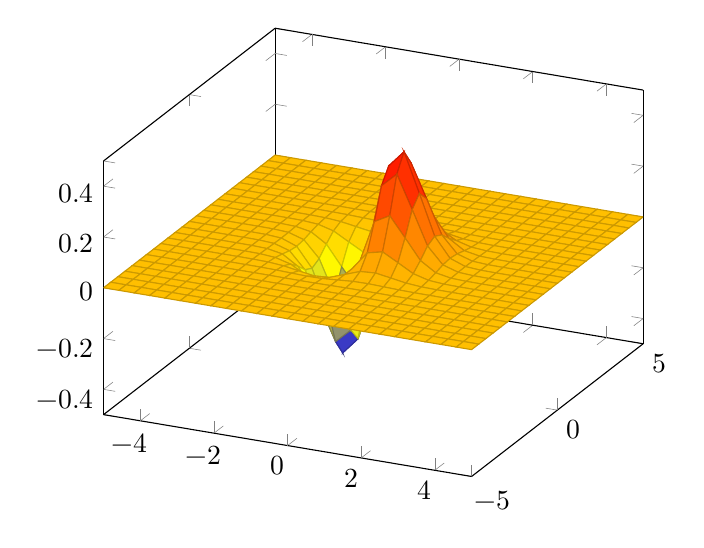
\begin{tikzpicture}
\begin{axis}
\addplot3[
    surf,
]
{exp(-x^2-y^2)*x};
\end{axis}
\end{tikzpicture}

\end{document}
